\chapter{Conceptual Design}
\label{ch:conceptualDesign}

\section{Requirements}
\label{ch:requirements}

In this chapter, the requirements for the synthetic data generation system will be first established.
The goal is to gather a systematic collection of requirements on which the success of the developed system can be measured.
Firstly, non-functional requirements will be explained before continuing with the functional requirements.


\subsection*{Non-Functional Requirements}

Non-functional requirements (or qualitative requirements) describe requirements and constraints on a system that governs how the functions specified in the functional requirements are to be performed \cite{broy2021EinfuehrungSoftwaretechnik}.
They focus on the question of how a system's functional requirements should be realized \cite{broy2021EinfuehrungSoftwaretechnik}.
The ISO-Norm 25010 \cite{iso/iecSystemsSoftwareEngineering} defines the base characteristics relevant for a software system's quality \cite{haoues2017GuidelineSoftwareArchitecture}.
The key elements of software architectures include functional suitability, reliability, performance efficiency, compatibility, usability, security, maintainability, and portability \cite{haoues2017GuidelineSoftwareArchitecture}.
Each of these is of different importance for each software system.
Additionally, \cite{vogelsang2019RequirementsEngineeringMachine} highlights that additional quality requirements might be necessary in the context of machine learning tasks, for which a standard has yet to be defined.
These could include (but are not limited to) quantitative targets (\ie measurable results), explainability, freedom from discrimination, legal and regulatory requirements, and data requirements.

This thesis focuses on a research prototype rather than a fully developed software system.
Therefore, only a subset of the aforementioned requirements are prioritized during development.
The following requirements R1 - R5 are the non-functional requirements for the software developed in this thesis:

%[TODO: GANZER ABSCHNITT AM ENDE AUF INHALTLICHE RICHTIGKEIT KORRIGIEREN]
\begin{description}
	\item[R1 - Functional Suitability:]
		Functional Suitability refers to "the degree to which a product or system provides functions that meet stated and implied needs when used under specified conditions" \cite[p. 219]{bass2013SoftwareArchitecturePractice}.
		In the context of this thesis, the system first needs to be able to generate synthetic data and needs to be able to show how different tabular processing techniques influence the performance of the overall synthesis approach.
		This performance should be measured across different similarity measures.
	\newpage
	\item[R2 - Maintainability:]
		Maintainability focuses on the "degree of effectiveness and efficiency with which a product or system can be modified by the intended maintainers" \cite[p. 220]{bass2013SoftwareArchitecturePractice}
		One of the core questions of this thesis is to compare different tabular processing techniques in diffusion models.
		For this, a variety of different approaches are intended to be compared.
		Hence, it is required that the code and software architecture is designed in a maintainable way, such that it can be easily extended with additional processing techniques, not only by the developer,
		but also for future researchers who might build upon the work of this thesis.

	\item[R3 - Performance efficiency:]
		In the context of deep learning, the program's performance is always essential since training, hyperparameter search, and inference usually demand a lot of computation time by nature.
		Consequently, the developed software should reduce unnecessary computations as much as possible.

	\item[R4 - Portability/Reproducibility:]
		Portability is usually referring to the extent of "effectiveness and efficiency with which a system, product, or component can be transferred from one hardware, software,
		or other operational or usage environment to another" \cite[p. 220]{bass2013SoftwareArchitecturePractice}.
		Since this thesis should encourage other researchers to reproduce and extend the developed codebase, the software should be able to run on other machines running a different operating system given a specified development environment,
		including packages used and their version numbers.
		In general, it is required that all results should be fully reproducible, given the parameters and the configuration of the experimental setups

	\item[R5 - Quantitative Targets:]
		It is required that the different model versions produced in the thesis are compared using metrics that are commonly used in the domain of tabular data synthesis.
		This should enhance the comparability to other approaches.
\end{description}


\subsection*{Functional Requirements}
\label{sec:func_requirements}
Functional requirements describe what the software system should do and which practical aspects must be implemented.
Please note that the software of \cite{kotelnikov2022TabDDPMModellingTabular} will be extended, which has consequences for certain functional requirements.

\begin{description}
	\item[FR1 - Data Import and Export:]
		The software shall support importing tabular data in the same format as specified in \cite{kotelnikov2022TabDDPMModellingTabular}.
		\textcite{kotelnikov2022TabDDPMModellingTabular} makes use of datasets, that are already separated into numerical, categorical, and target columns, each saved in a NumPy \cite{harris2020array} array.
		Additionally, the datasets that will be imported have to be separated into training, validation, and testing sets.
		For the NumPy arrays to be imported, they need to be of file type ".npy".
		Synthetic data produced by models shall be saved in the same data segmentation format as the imported data.

	\item[FR2 - Tabular Processing:]
		The software shall support tabular data processing techniques that are able to encode and decode tabular data.
		An \textit{IdentityProcessor} that has no effect is required to be implemented to test models without any tabular processing mechanism.
		Additional data transformation techniques proposed by \cite{kotelnikov2022TabDDPMModellingTabular}, including normalization or categorical encoding, shall still be supported as intended by the authors.
		Adding new tabular processing mechanisms shall not affect other existing tabular processing mechanisms. This requirement implies several sub-requirements: 

		\item[FR2.1 - Tabular Processing Fit:]
		If necessary, a Tabular processing mechanism should be able to be fitted according to the data.
		However, it is required that the tabular processing mechanism only receives training and validation data and does not have access to the test data.

		\item[FR2.2 - Tabular Processing Transform:]
		Each Tabular processing mechanism needs to transform the raw data into a specified format.

		\item[FR2.3 - Tabular Processing Inverse Transform:]
		Each Tabular processing mechanism \\needs to be able to inversely transform data back into its original form.

		\item[FR3 - Diffusion Process Configuration:]
		Several experiments with different model configurations will be tested.
		The software shall allow users to configure the diffusion process by specifying parameters such as the number of iterations, batch size, sampling size, and others.

		\item[FR4 - Training, Tuning, Sampling, Evaluation:]
		The software shall support the training of various model versions, including the TabDDPM diffusion model, variations of TabDDPM and other non-diffusion baseline models.
		The software shall allow finding of suitable hyperparameters in a specified hyperparameter search space.
		During training, relevant metrics and loss values shall be saved.
		The software shall generate synthetic samples from the trained diffusion model during the sampling process, where the user specifies the number of synthetic samples to be generated.
		The software shall handle the evaluation of synthetic data in multiple ways.
		Firstly, the existing evaluation framework of \cite{kotelnikov2022TabDDPMModellingTabular} shall remain.
		Additionally, a similarity evaluation shall be implemented according to \cite{chundawat2022UniversalMetricRobust}.
		Lastly, the software should also produce visualizations of certain properties of the synthetic data to allow a visual comparison with the same properties of the real data, for example, to allow for a comparison of distributions of columns.

	\item[FR5 - Modularity:]
		The individual software components (tabular data processing, training, sampling, evaluation) shall be implemented in such a way,
		that they are easily replaceable by alternatives (for tabular data processing) or shall be executed individually (training, sampling, evaluation).
		For example, sampling synthetic data shall be separated from the training so that not every sampling process requires training a model from the start.
\end{description}


\section{Existing Code Base}
\label{ch:conceptualDesign-existingCodeBase}

The software \cite{akim2023TabDDPMModellingTabular} used in this experiment was programmed in the programming language python \cite{van1995python} and is based upon the work of \cite{kotelnikov2022TabDDPMModellingTabular}.
It is changed and modified according to the needs of the experiments.
This section will first explain the architecture of the existing code base before introducing the proposed adaptations in the next section.

\begin{figure}[h]
	\centering
	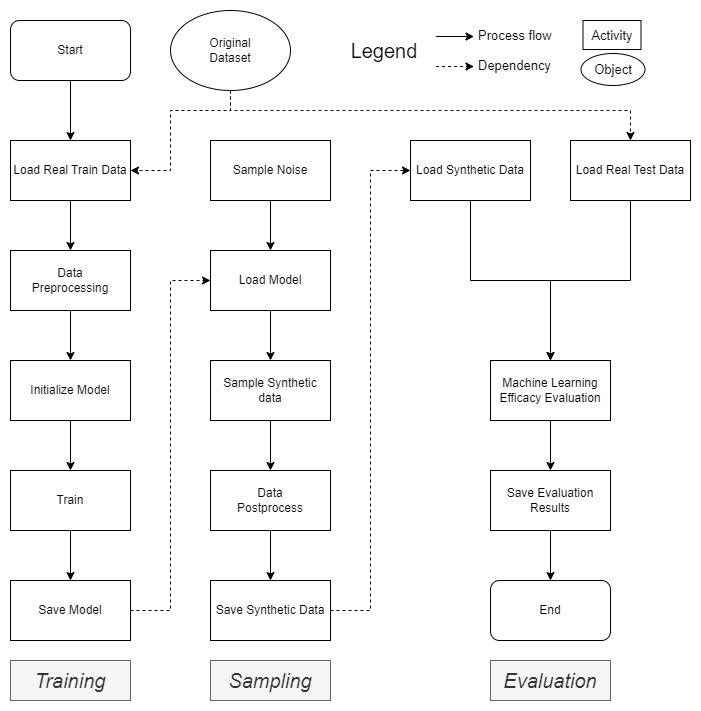
\includegraphics[width=0.8\textwidth]{images/Overall_original.png}
	\caption[Overview Original Software]{Overview synthetic data generation process in \cite{akim2023TabDDPMModellingTabular}}
	\label{fig:overall_original}
\end{figure}


\subsection{Original Implementation}
\label{ch:conceptualDesign-existingCodeBase-originalImplementation}

\textcite{akim2023TabDDPMModellingTabular} provide a software implementation for their proposed TabDDPM.
This implementation consists of multiple scripts and implements several of the functional requirements listed in \autoref{sec:func_requirements}, including FR1, FR4, FR5, and parts of FR4.
This section will explain what kind of software was already provided by \cite{kotelnikov2022TabDDPMModellingTabular} and explain important architectural design choices.

\subsubsection[]{Software Procedure}
\label{ch:Software_Procedure}

An overview of how the overall process in this synthetic data generation approach is done can be seen in \autoref{fig:overall_original}.
The whole software process can be roughly summarized into three parts, the training, the sampling, and the evaluation.
In the training, real training data is taken from the original dataset.
This training data is preprocessed, according to a predefined preprocessing strategy that may vary from dataset to dataset (compare \autoref{sec:preprocessing}).
After preprocessing, the diffusion model is initialized and trained to learn the underlying joint distribution of the training data.
Once the training is finished, the sampling of new synthetic data can be executed.
The previously trained model is loaded and synthetic data will be produced by denoising previously sampled noise.
The synthetic data will be in the same format as the training data after it has been preprocessed.
Hence, the synthetic data will be postprocessed by inverting the preprocessing, such that the synthetic data will be in the same format as the raw training data.
As a last step, the synthetic data will be evaluated. 
For this, the held-back real test set will be loaded.
With the real test set and the synthetic dataset sharing the same data format, a machine learning efficacy evaluation (compare \autoref{ch:preliminaries-machineLearningEfficacy}) is performed to compare the two datasets.
Ultimately, the results of this evaluation are saved and can be interpreted by the user.

\subsubsection[]{Scripts}
\label{ch:scripts}

The implementation \cite{akim2023TabDDPMModellingTabular} already provides the necessary scripts that allow for an
easy training, sampling, evaluation, and hyperparameter tuning for their proposed TabDDPM model.
Additional non-diffusion baseline models the TabDDPM is compared against are supported as well.
The functionality of the most important scripts can be summarized in the following way:

\begin{description}
	\item[train.py:]
		The script "train.py" is responsible for the training of the diffusion model. 
		It accepts configuration parameters that guide the training process. 
		Initially, it loads the designated dataset and carries out preprocessing as per the given configuration. 
		Subsequently, it initializes the necessary class instances and starts the training loop. 
		Once the training loop is finished, the script saves the trained model along with its loss history.

	\item[sample.py:]
		The script "sample.py" carries out the task of sampling from a pre-trained diffusion model. 
		It takes in specific configuration parameters that are used during the sampling procedure. 
		This script starts by loading a pre-trained model and generating samples from it. 
		These new samples are then modified in accordance with the inverse of the preprocessing defined in the configuration.
		Once the transformation is complete, the resulting samples are saved.

	\item[\text{eval\_[catboost\textbar mlp\textbar simple].py:}]
		The scripts "eval\_catboost.py", "eval\_mlp.py", and \\"eval\_simple.py" evaluate a synthetic dataset based on machine learning efficacy. 
		In this process, a machine learning model, chosen by the user, is trained on either real or synthetic data, as specified in the configuration. 
		The model's performance is then assessed on the real test set by computing a set of metric scores.

	\item[pipeline\_*.py\footnotemark:]
		The scripts, denoted as "pipeline\_*.py", define the full processing pipeline, which includes the processes of training, sampling, and evaluation. 
		They ensure that each function within the pipeline correctly receives its necessary attributes from the configuration. 
		These scripts also provide the flexibility to execute specific portions of the pipeline individually.
		\footnotetext[1]{Each implemented baseline model (SMOTE, TVAE, CTABGAN, CTABGAN+) has its own implementation as pipeline\_\textit{modelName}.py.}

	\item[tune\_*.py\footnotemark:]
		The "tune\_*.py" scripts are generally responsible for the hyperparameter tuning process.
		It starts by defining a hyperparameter search space (see \cite[Table 1, p. 4]{kotelnikov2022TabDDPMModellingTabular} and \cite[Table 7-11, p. 13 f.]{kotelnikov2022TabDDPMModellingTabular}).
		Next, an objective function is defined that is maximized for 50 trials through the Optuna framework \cite{optuna_2019}.
		Within the objective function, a set of hyperparameters is selected from the search space.
		These selected hyperparameters are used to invoke \textit{pipeline.py}, which initiates the model training
		Afterward, for five different random initializations, \textit{pipeline.py} is called to sample and evaluate the model, creating, and assessing five different synthetic dataset versions.
		In each training, sampling, and evaluation, the training and validation set are redistributed and shuffled to implement some form of cross-validation \cite{kohavi2001StudyCrossValidationBootstrap}.
		The average evaluation score (machine learning efficacy based) of the five synthetic dataset versions is returned as the objective that Optuna tries to maximize.
		After optimization, the best hyperparameter configuration is saved.
		If the user has set an \textit{- - eval\_seeds} flag, a final evaluation of the best-found model will be started by calling \textit{eval\_seeds.py}.
		\footnotetext[2]{Each implemented baseline model has its own implementation as tune\_\textit{modelName}.py.}
		
	\item[eval\_seeds.py:]
		The "eval\_seeds.py" script's purpose is to perform an extensive evaluation, given a trained model.
		The script starts by loading the pre-trained sampling model \\([TabDDPM|SMOTE|CTABGAN|CTABGAN+|TVAE]).
		Given the sampling model, $n\_datasets$ synthetic datasets will be produced depending on the specified evaluation parameters by calling the sampling script in the respective \textit{pipeline\_*.py} script.
		For each produced dataset, evaluation is performed using a predefined evaluation model ([Catboost|MLP]) for a predefined number of random initializations.
		Ultimately, the average metrics are calculated over all performed runs, reported, and saved.
\end{description}

In summary, to get a fully optimized diffusion model with an extensive evaluation, the user just has to run the \textit{tune\_ddpm.py} script with the \textit{- - eval\_seeds} flag.
A detailed activity diagram for each script can be found in the Appendix \ref{A:activity_diagrams}.

\subsubsection[]{Configuration}

In order to start one of the above scripts, a configuration file has to be specified, detailing the most important parameters for training, sampling, and evaluation.
For example, \autoref{lst:configuration} shows how such a configuration file could look like and which parameters need to be specified.
The file is stored as a \gls{toml} \glsadd{tomlaccr} file (short for "Tom's Obvious, Minimal Language") \cite{preston-werner2021TOMLTomObviousa}, which contains sections, indicated by squared brackets. 
Within these sections, key-value pairs define configuration options.

\begin{lstlisting}[label={lst:configuration}, caption={Example Configuration File}]
    parent_dir = "exp/adult/check"
    real_data_path = "data/adult/"
    num_numerical_features = 6
    model_type = "mlp"
    seed = 0
    device = "cuda:0"

    [model_params]
    num_classes = 2
    is_y_cond = true

    [model_params.rtdl_params]
    d_layers = [
        256,
        256,
    ]
    dropout = 0.0

    [diffusion_params]
    num_timesteps = 1000
    gaussian_loss_type = "mse"
    scheduler = "cosine"

    [train.main]
    steps = 1000
    lr = 0.001
    weight_decay = 1e-05
    batch_size = 4096

    [train.T]
    seed = 0
    normalization = "quantile"
    num_nan_policy = "__none__"
    cat_nan_policy = "__none__"
    cat_min_frequency = "__none__"
    cat_encoding = "__none__"
    y_policy = "default"

    [sample]
    num_samples = 216000
    batch_size = 10000
    seed = 0

    [eval.type]
    eval_model = "catboost"
    eval_type = "synthetic"

    [eval.T]
    seed = 0
    normalization = "__none__"
    num_nan_policy = "__none__"
    cat_nan_policy = "__none__"
    cat_min_frequency = "__none__"
    cat_encoding = "__none__"
    y_policy = "default"
\end{lstlisting}


The key \textit{model\_type} refers to the model that should approximate the noise in the reverse noising process.
Most parameters are self-explanatory, controlling one specific part of the pipeline.
For example, all \textit{model\_params} specify different relevant aspects for instantiating the model.
Inside the \textit{model\_params} section, the \textit{num\_classes} key indicates the number of possible target classes the given dataset has, and \textit{is\_y\_cond} indicates if the dataset is a classification (=\textit{True}) or regression dataset (=\textit{False}).
The \textit{model\_params.rtdl\_params}\footnote{rtdl is an abbreviation for the python library \cite{gorishniy2021RevisitingDeepLearning} from which the \gls{mlp} model architecture was used.} specify the \glp{mlp} architecture, by controlling the number of layers and the amount of dropout.
As the name suggests, the keys inside the \textit{diffusion\_params} section control the diffusion process.
Noteworthy are the \textit{train.T} and \textit{eval.T} sections, whose keys define how preprocessing is done at the beginning of training and evaluation, respectively.
The \textit{eval.type} section keys are useful to further specify the kind of evaluation that will be executed.
The machine learning efficacy model is determined by the \textit{eval\_model} key and is, in this example, set to the CatBoost model.
To control what kind of data will be evaluated, the \textit{eval\_type} key can be set to either "real" or "synthetic".
If the value is set to "real", the real training data is loaded and compared to the real test data, as if it was synthetic data.
This setting allows the creation of baseline metric scores against which synthetic values are compared.
As this is usually done only once per dataset, \textit{eval\_type} is usually set to "synthetic" to calculate metric scores for the newly created synthetic data.
This configuration structure allows to efficiently perform a variety of experiments with different key configurations by simply changing the configuration file and inputting it into the next experimental run.

\subsubsection[]{Dataset Segmentation}
\label{sec:data_format}
The authors provide access to 12 different datasets, which have already been cleaned and formatted by a program provided by \textcite{gorishniy2023EmbeddingsNumericalFeatures}.
In order to use and process the data, the software of \cite{kotelnikov2022TabDDPMModellingTabular} is built towards processing the data that was segmented as specified by \textcite{gorishniy2023EmbeddingsNumericalFeatures}.
For the purpose of clarity in this thesis, any future reference to "data segmentation" will refer to the separation of a dataset into multiple parts, detailed as follows:

Each dataset contains data separated into multiple subcomponents, saved as individual files.
To create these subcomponents, the columns of the dataset are manually classified into categorical, numerical, ("X") and target ("y") columns.
Secondly, the dataset records are distributed into a training, validation, and testing set.
Therefore, each dataset is separated into nine parts, conforming to the subsequent naming convention:
X\_[cat|num]\_[train|val|test].npy and for the target y\_[train|val|test].npy

Additionally, a \textit{info.json} file is provided, containing the necessary information for handling the data.
In \autoref{lst:info}, one can see how such an info-file contains the information on how the splits mentioned above have been done and what kind of task this dataset usually has (it is differentiated between binary classification (binclass), multiclass classification (multiclass), and regression (regression)).
\begin{lstlisting}[label={lst:info},caption={Example Data-info File}]
    {
    "name": "Adult",
    "id": "adult--default",
    "task_type": "binclass",
    "n_num_features": 6,
    "n_cat_features": 8,
    "test_size": 16281,
    "train_size": 26048,
    "val_size": 6513
    }
\end{lstlisting}
Inside the code of TabDDPM \cite{akim2023TabDDPMModellingTabular}, a custom dataset class provided by the author handles any dataset that follows the above naming convention and provides a matching information file.

\section{Proposed Concept}
\label{ch:conceptualDesign-changes}

Changes to the current architecture have been made to answer the research questions specified in \autoref{ch:intro-goals}.
\autoref{fig:Overall_changed} shows that the overall synthesis process does not deviate much from \autoref{fig:overall_original}.
Changes are highlighted in green and affect each step in the diffusion process: the training, sampling, and evaluation step.
For a detailed overview of how each individual scripts changed, please refer to Appendix \ref{A:activity_diagrams}.

\begin{figure}[h]
	\centering
	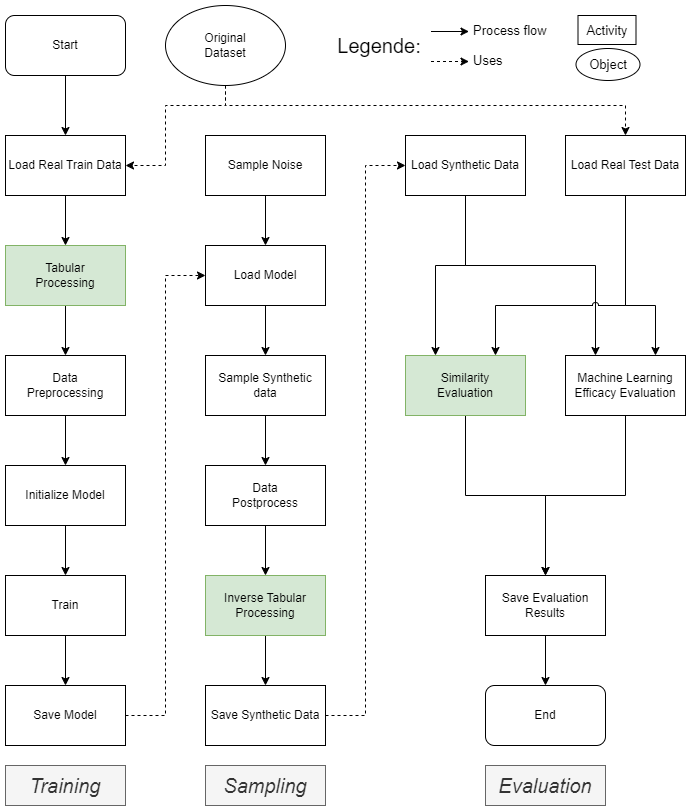
\includegraphics[width=0.8\textwidth]{images/Overall_changed.png}
	\caption[Overview Software Changes]{Overview of proposed synthetic data generation process changes (highlighted in green)}
	\label{fig:Overall_changed}
\end{figure}

\begin{description}
	\item[C1-Tabular Processing:] To test the effect of different tabular processing techniques, a "Tabular processing" step is required before training the diffusion model.
		Within this processing, the raw data is transformed according to the defined tabular processing strategy.
		The tabular processing data output format needs to be the same as before the transformation, described in \autoref{sec:data_format}, to ensure
		that the remaining pipeline remains functional and keeps changes to the original code minimal.
	\item[C2-Inverse Tabular Processing:] Similar to the data preprocessing, which requires an inverse data postprocessing, to turn the data back into its original format and scale, the same is necessary for the tabular processing.
		Since the model is trained on data that has been transformed according to the tabular processing mechanism, the diffusion model will produce data in the same format.
		Consequently, the synthetic data must be transformed back by an inverse function of the tabular processing mechanism before it is evaluated.
	\item[C3-Similarity Evaluation:] Lastly, an extended evaluation of the synthetic data's similarity to the real data should be performed.
		For this, the original machine learning efficacy evaluation remained unchanged.
		However, the evaluation pipeline is extended by a similarity evaluation that does not only calculate a unified score, TabSynDex \cite{chundawat2022UniversalMetricRobust}, but also reports other metric results that are of interest.
		Hyperparameters of the generation models can also be tuned towards the TabSynDex score.
		In addition to the numeric metric results, several visualizations comparing real and synthetic data will be generated.
\end{description}

%<-------------
\subsection{Tabular Processing Criteria}
\label{ch:Concept-criteria}

The main source for finding the processing mechanisms should be academic literature, where said mechanism has been successfully applied to a related problem.
The selection of which tabular processing mechanisms are realized heavily depends on the requirements defined in \autoref{sec:func_requirements}.

For a tabular processing mechanism to be used, the following conditions must be met:

\begin{description}
	\item[1. Reversibility:] the tabular processing mechanism must not only transform the data into a different format, but it also must be able to revert the transformation
	      such that the data can be transformed back into its original form.
	\item[2. Compatibility:] the data must be able to be separated into numerical and categorical parts after the transformation
	      since the remaining code expects data in this format, as specified in \autoref{sec:data_format}.
	\item[3. Complexity:] the time it takes to transform the data should be within a reasonable timeframe. They shall not add too much computation time to the already extensive model-tuning process.
	\item[4. Availability:] due to the limited time frame of this thesis, the code for the mechanisms should be publicly available (or could be implemented within a reasonable timeframe).
\end{description}

\subsection[]{Evaluation}
\label{ch:conceptualDesign-Evaluation}
The evaluation framework shall contain multiple evaluation aspects.
Firstly, the existing machine learning efficacy using a CatBoost model proposed by \cite{kotelnikov2022TabDDPMModellingTabular} shall be executed and remain untouched.
In addition, the TabSynDex \cite{chundawat2022UniversalMetricRobust} similarity will be performed in each evaluation.
Machine learning efficacy that is based upon an \gls{mlp} or using a set of classification models will not be performed for the following reasons:
\begin{enumerate}
	\item \cite{kotelnikov2022TabDDPMModellingTabular} argues convincingly that machine learning efficacy not based on CatBoost is less informative compared to the CatBoost counterpart.
	\item The TabSynDex metric contains a machine learning efficacy metric based upon a set of models.
\end{enumerate}
Consequently, machine learning efficacy will be evaluated twice in each evaluation, once based on CatBoost and once inside the TabSynDex metric using a set of standard machine learning models.

Lastly, for a visual evaluation, several plots indicating the similarity of the synthetic data to the real data shall be generated using the implementation of \textcite{brenninkmeijer2019GenerationEvaluationTabular}.
If necessary, modifications to the plots may be required.

% ''TODO:
% ML efficacy like in the original paper + Tabsyndex similarity score + similarity score of anderes paper (+bilder von denen)

% aufzählen was alles klassische ml efficacy is (acc, f1, roc) und was sim_score werte sind''